\chapter{Related Work}
\label{chapter:related-work}

% Should be around 20 pages

Interactive image visualization techniques have been explored for some time now, many of them related to image organization or retrieval in large collections. There have been some interesting ideas across the board and we will now take a look at some of them.


\section{Related work}

\subsection{Visual guided navigation for image retrieval} % (fold)
\label{sub:Qiu}

Qiu et al. \cite{Qiu:2007p1207} explore the requirements of a system intended for visualizing large photo collections. They identify as the two most important requirements, the first being an easy to use \ac{UI}, that gives clean information to the user and helps to create a mental image of the whole collection helping him to navigate on the collection. The second requirement is responsiveness because while image processing can be an heavy task, the user needs to be able to interact with the interface and he won't use the application if it's slow. 

\begin{figure}[ht]
	\centering
		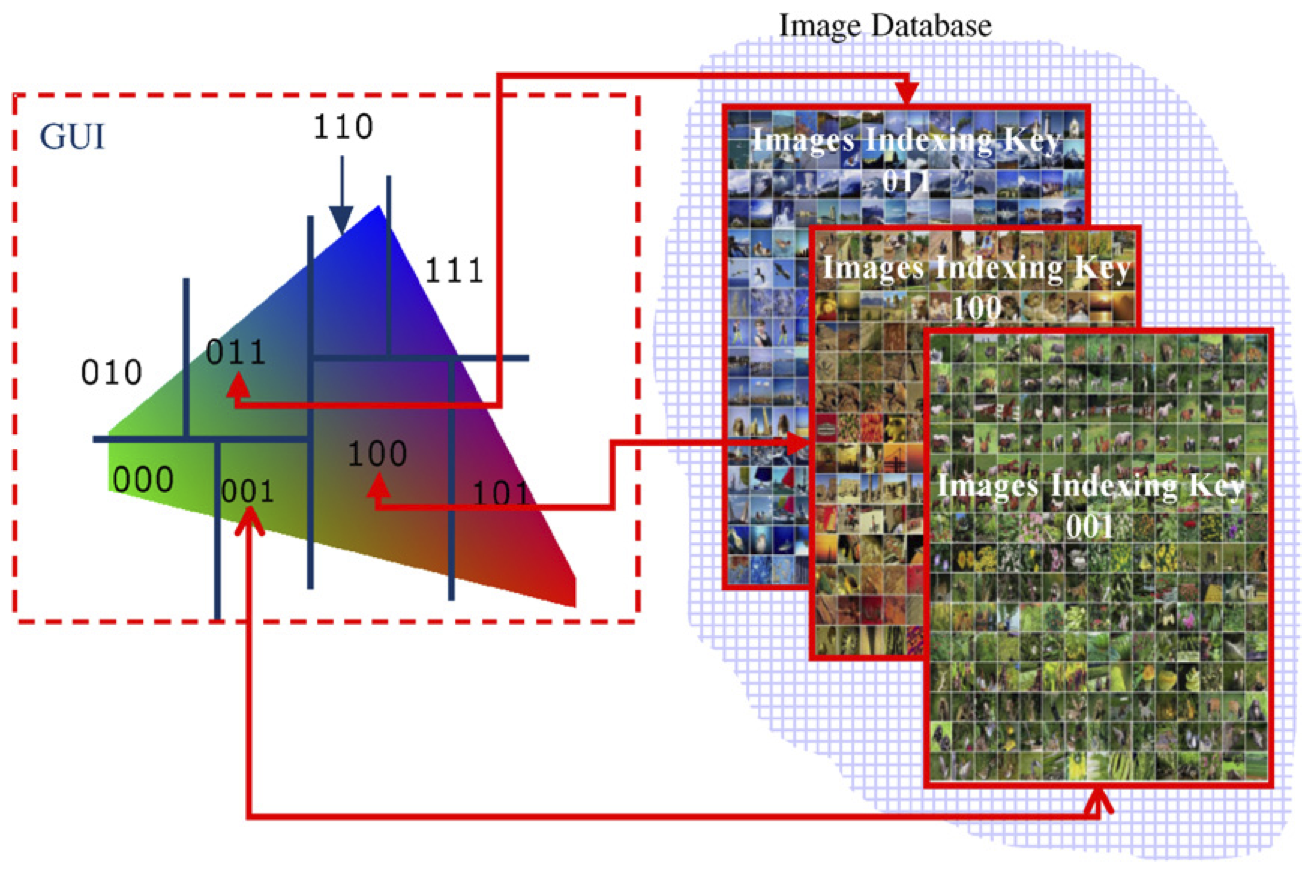
\includegraphics[width=0.6\columnwidth]{imgs-RelatedWork/Qiu-2007p1207.png}
	\caption[Chromacy diagram and color related images, from the work of Qiu et al.]{The chromacy diagram is split in parts and each image belongs to one of this parts. The diagram is part of the \ac{UI} and  when navigating through the diagram, only the images related to that part are shown.}
	\label{fig:qiu1}
\end{figure}

The system shows all the photos arranged by color, just as many others like it. The difference is the process in use. Instead of calculating distance vectors based on the histogram of each image, this approach classifies each image with a simple description, like an average of its colors, and arranges them by that value, on a color map (\fig{qiu1}). The process is much faster, but is also more error prone, specially on photos without a clear main color.

Their tests show they achieved good responsiveness and better results than using a file explorer.

% section Qiu (end)

\subsection{Does organization by similarity assist image browsing?} % (fold)
\label{sub:Rodden}
\begin{figure}[ht]
	\centering
		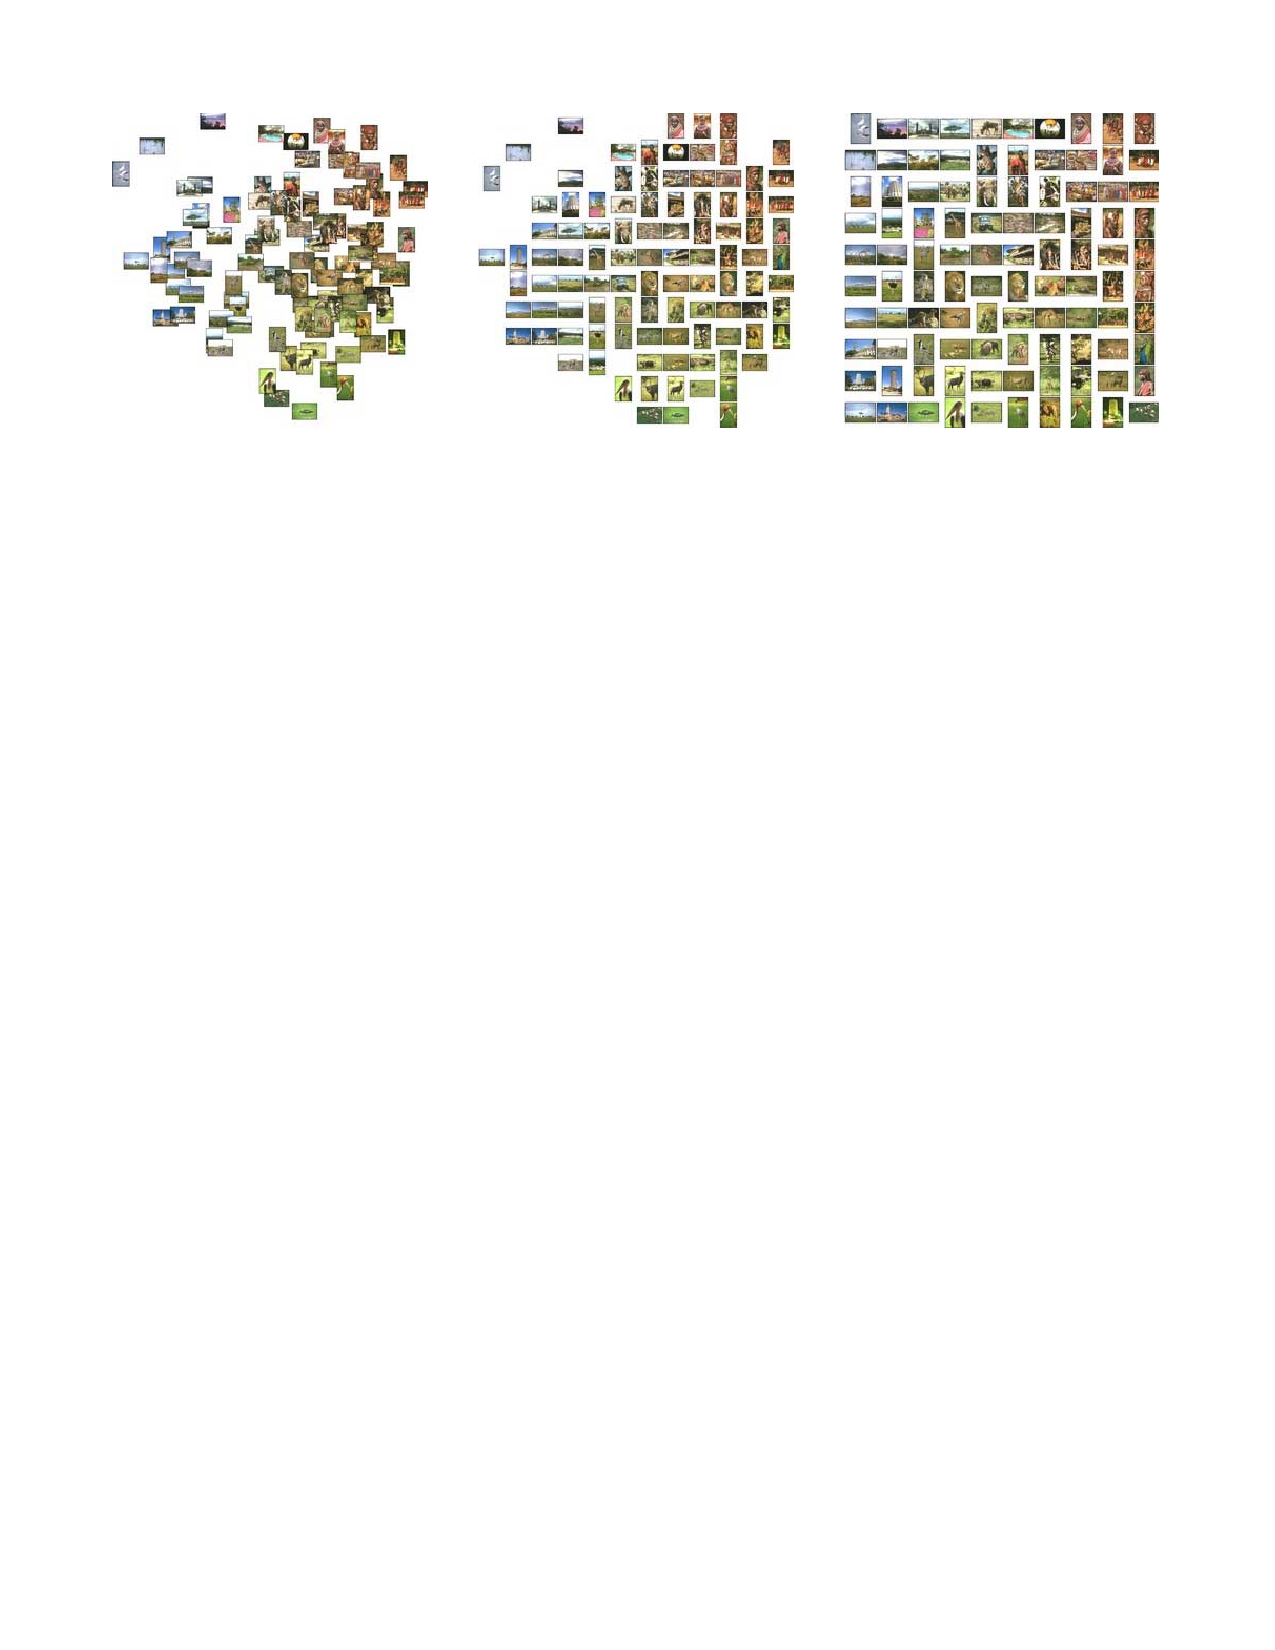
\includegraphics[width=\textwidth]{imgs-RelatedWork/Rodden1}
	\caption[Three arrangements of 100 images of Kenya, based on visual similarity, from the work of Rodden and Sinclar]{Three arrangements of 100 images of Kenya, based on visual similarity. On the left is the arrangement with overlap, in the middle a 12x12 grid (which removes the overlap while preserving some of the structure), and on the right a 10x10 grid (which maximises the thumbnail size).}
	\label{fig:Rodden1}
\end{figure}

The aim of this work by Rodden and Sinclar \cite{Rodden:2001p731} was to evaluate how photo organization by similarity (\fig{Rodden1}) could benefit a user looking for images. Some users tested an application that could show the same images both in a random and in an organized by similarity way. This organization by similarity was based on a rough description of the images, but it could be other descriptors.

The results differ if the user knows what he's looking for or not. In case he does, being able to filter only the relevant images makes it quick to find the ones that matter. This obviously depends on the quality of the labeling. Users reported that sometimes the similar images appear to merge.

In case the user doesn't know what he's looking for, the random approach might be helpful because the strong images usually contrast to their neighbors and thus appear to stand out.

For some people, having access to different arrangements of the same set of images is useful, although the source of the individual differences still needs to be determined.

% section Rodden (end)


\subsection{Browsing large collections of images through unconventional visualization techniques} % (fold)
\label{sub:Porta}

\begin{figure}[!htb]
  \begin{subfigmatrix}{2}
    \subfigure[Spot display]{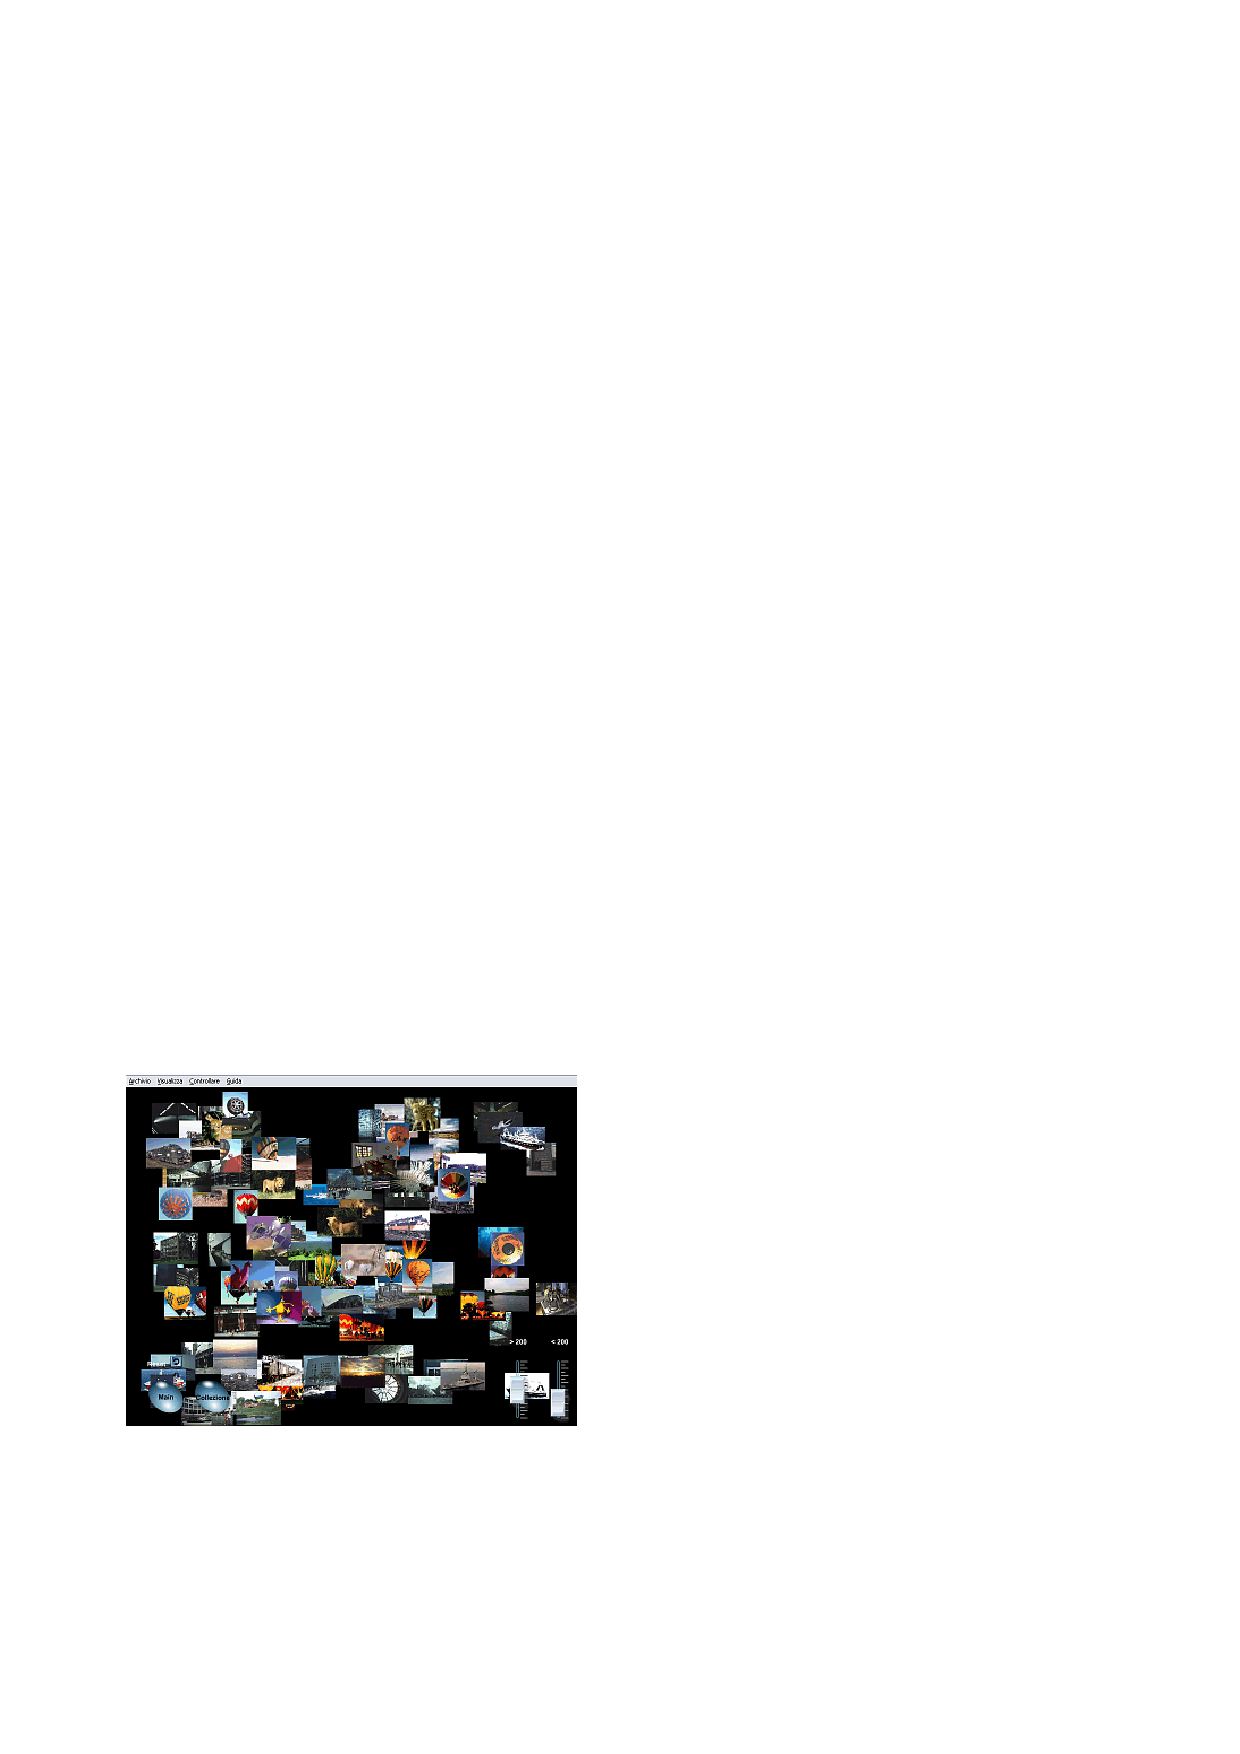
\includegraphics[width=0.49\linewidth]{imgs-RelatedWork/Porta-spot}\label{fig:porta-spot}}
    \subfigure[Shot display]{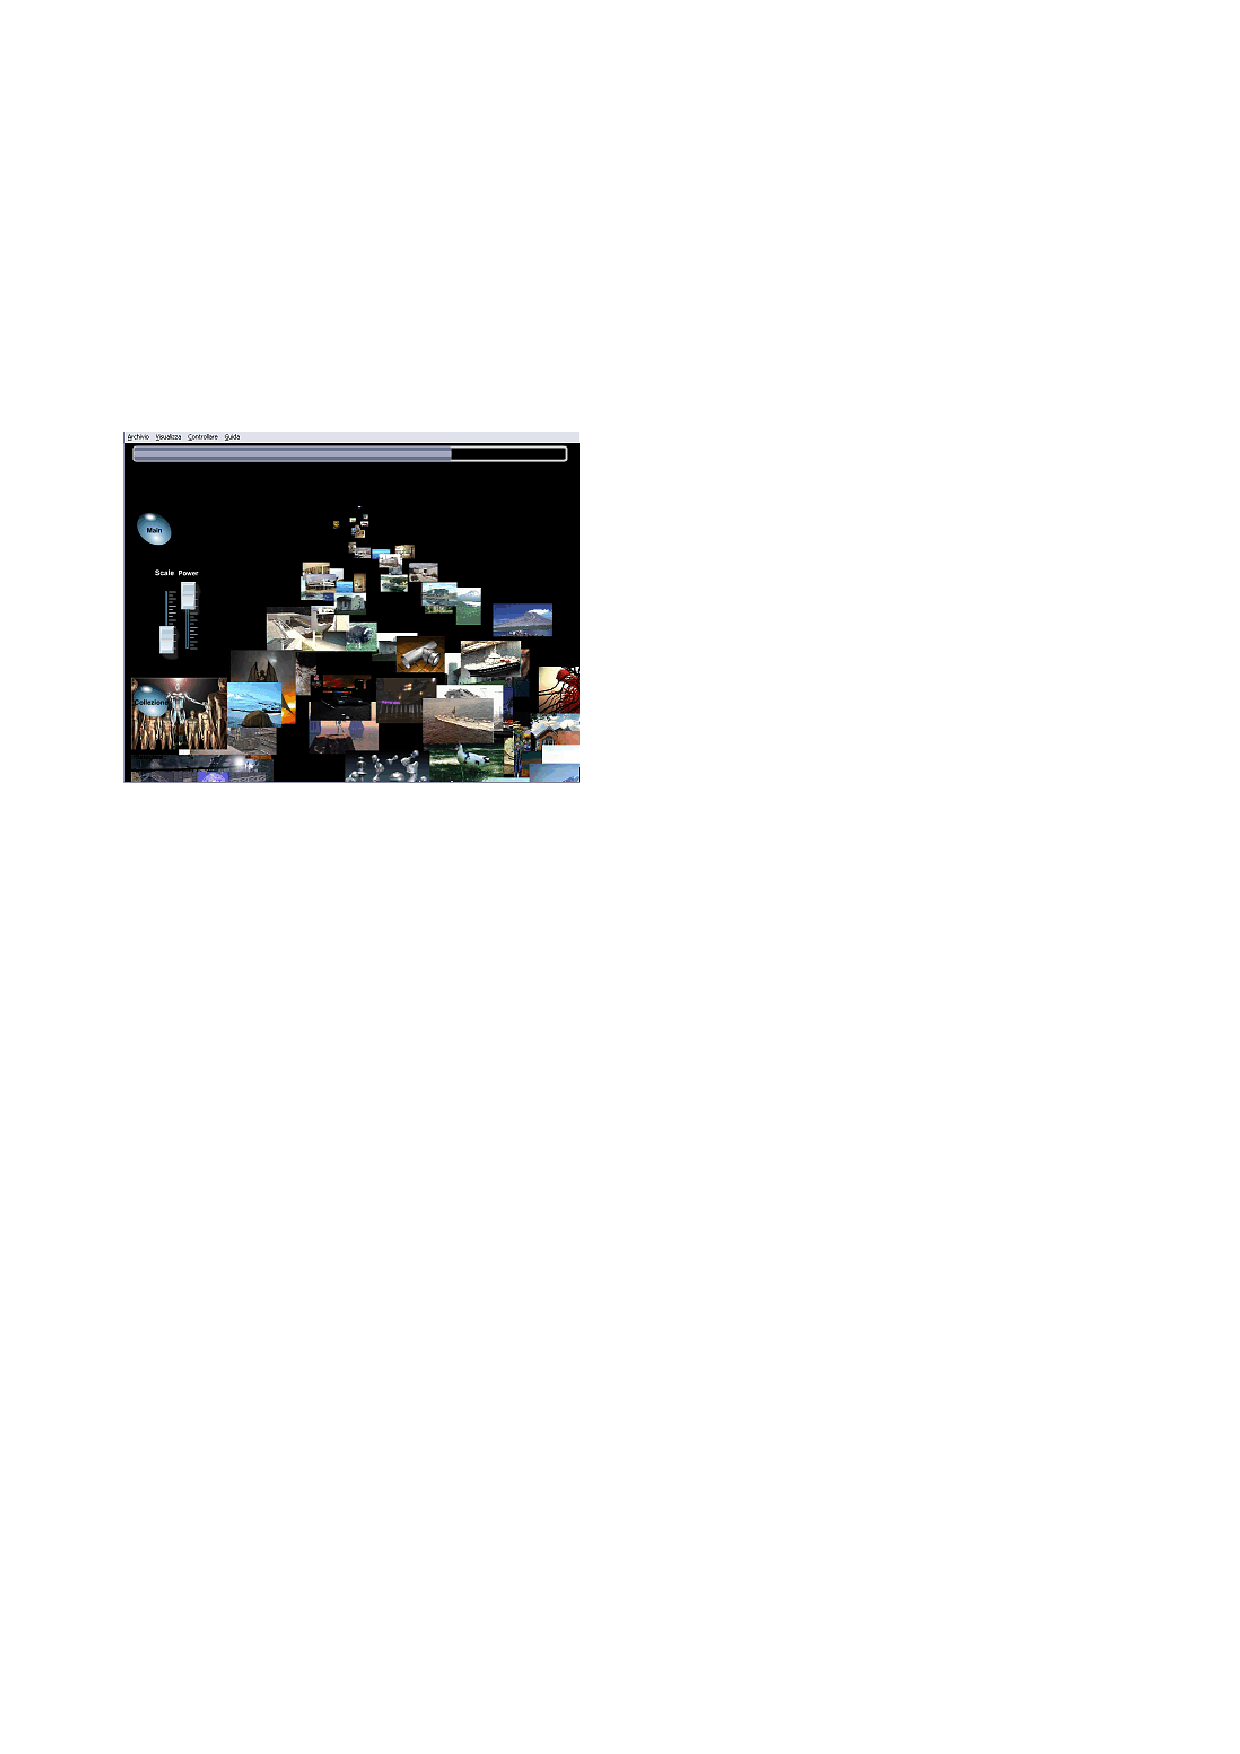
\includegraphics[width=0.49\linewidth]{imgs-RelatedWork/Porta-shot}\label{fig:porta-shot}}
  \end{subfigmatrix}
  \caption{The two better visualizations from Porta's work.}
  \label{fig:porta}
\end{figure}


Porta \cite{Porta:2006p416} describes a few visualization methods for large collections of images and tests them with users. The purpose is to find ways or metaphors that provide a good visualization experience in terms of time spent and quality of the visualization.

Some of the various techniques were the simple image grid view, a grid view with variable and independent height and width (EIB), a view that animates images like they were shot from a distance and get closer to the user called Shot (\fig{porta-shot}), a view where images quickly appear on random positions on screen named Spot (\fig{porta-spot}), and some other less commons like one that simulates a cylinder created with images (Cylinder), and others less relevant (Rotor, Tornado and Tornado of Planes).

The testing was based on the efficiency of users searching for specific images on a collection of a thousand photos. The Spot view was the best, followed the Shot, Cylinder finally the common grid view. The other views got scores near or below the grid view.

% section Porta (end)

\subsection{A comparison of static and moving presentation modes for image collections} % (fold)
\label{sub:Cooper}

This paper by Cooper et al. \cite{Cooper:2006p543} is not about large libraries, but about what kind of interfaces for image showing has greater success of user recognition and preference (\fig{Cooper1}).

With the help of eye-tracking techniques and user preference, the authors determined that static images are better than moving ones because makes them easier to recognize and avoid some user confusion.

\begin{figure}[ht]
	\centering
		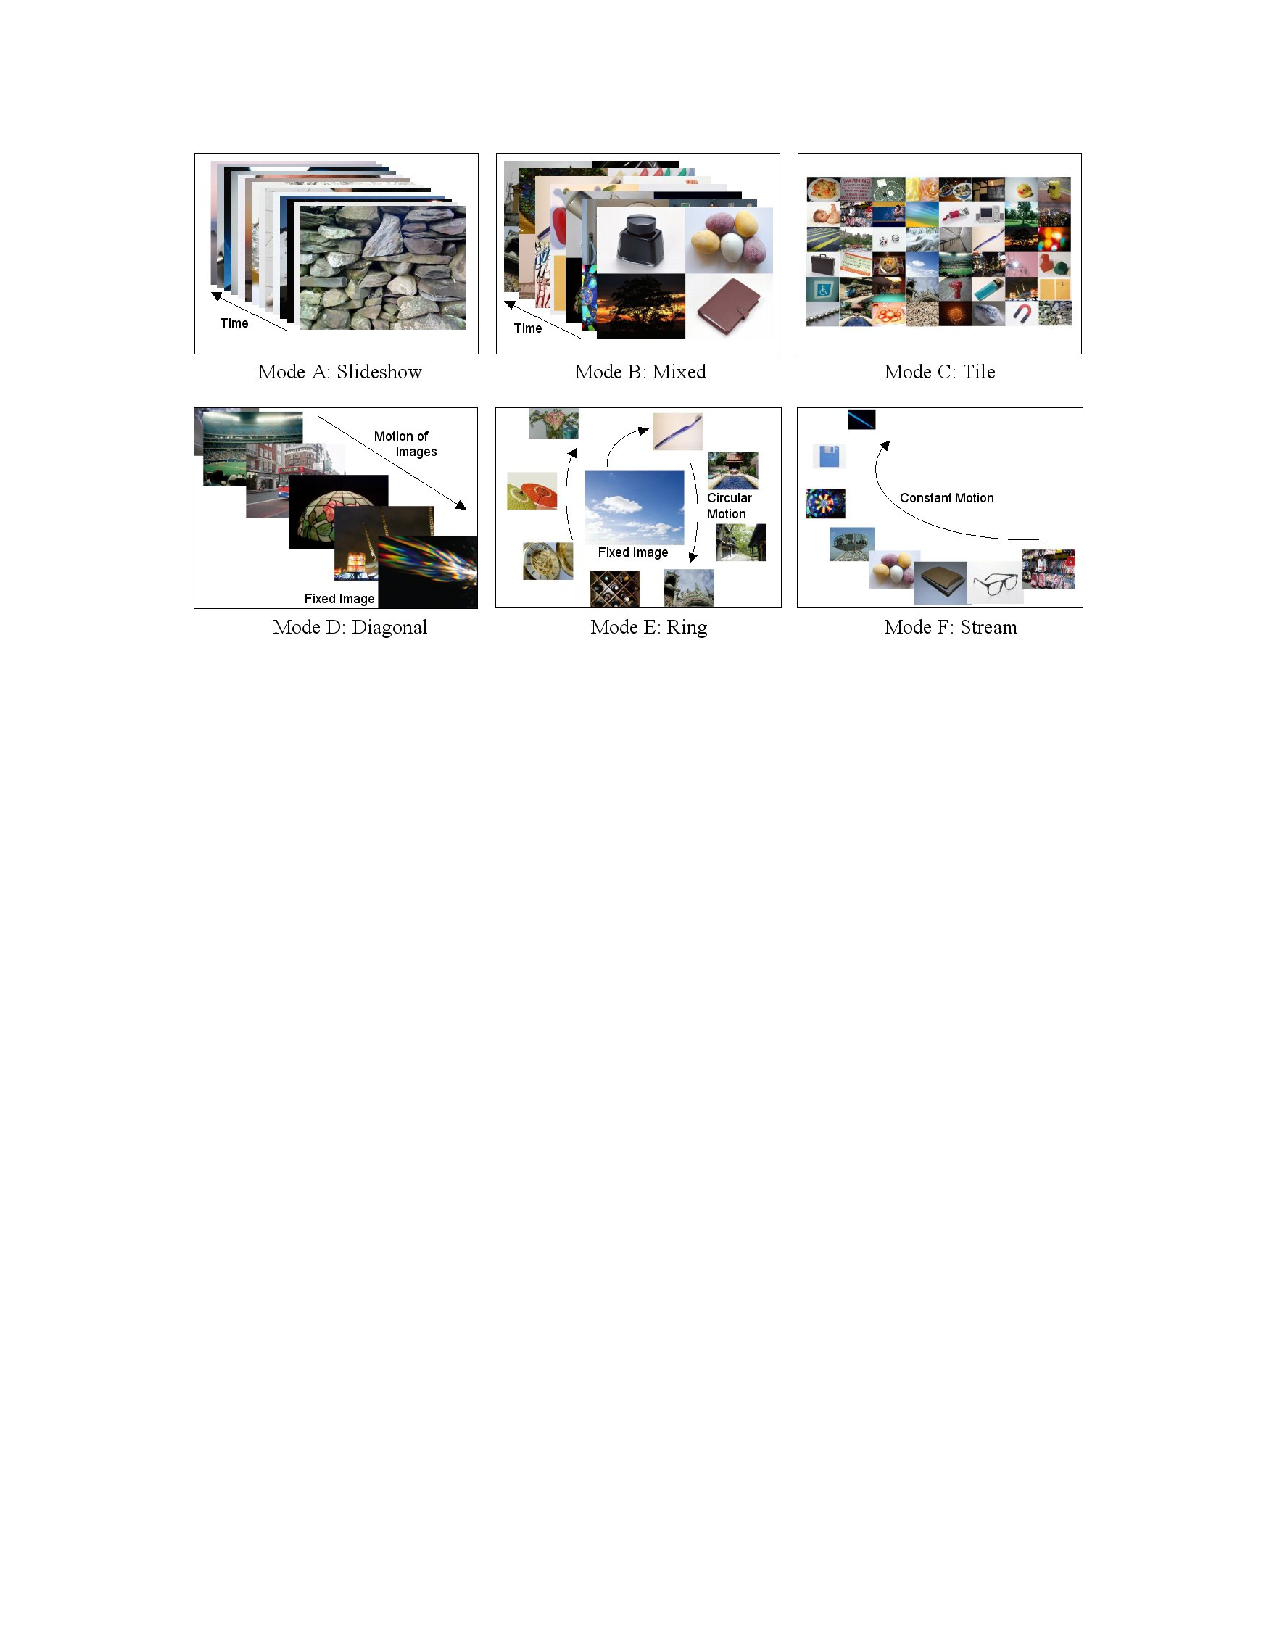
\includegraphics[width=\textwidth]{imgs-RelatedWork/Cooper1}
	\caption{The six rapid serial visual presentation modes used in the experiments}
	\label{fig:Cooper1}
\end{figure}
% section cooper (end)

\subsection{Organizing and browsing photos using different feature vectors and their evaluations} % (fold)
\label{sub:Strong}

Although it doesn't mention why, Strong \cite{Strong:2009p413} focuses on the better experience provided by color organization of a large image collection (\fig{Strong1}).

A \ac{SOM} is used to display the images on the screen featuring zooming, panning and sorting capabilities. The work is then based around the various methods used to determine the images' similarity.

Simpler methods are based on color histograms, which aren't affected by rotations or scales but, by not having spacial information on colors, allows very different images be closer together.

Other methods rely on gradients which contain spatial information and, therefore, are sensitive to image contents, but not color.
In general, the best methods were found to be the hybrid ones, where both color histograms and gradients are used to classify the images.
No user testing is made in this project, neither is the speed of image categorization referred about the methods used.

\begin{figure}[ht]
	\centering
		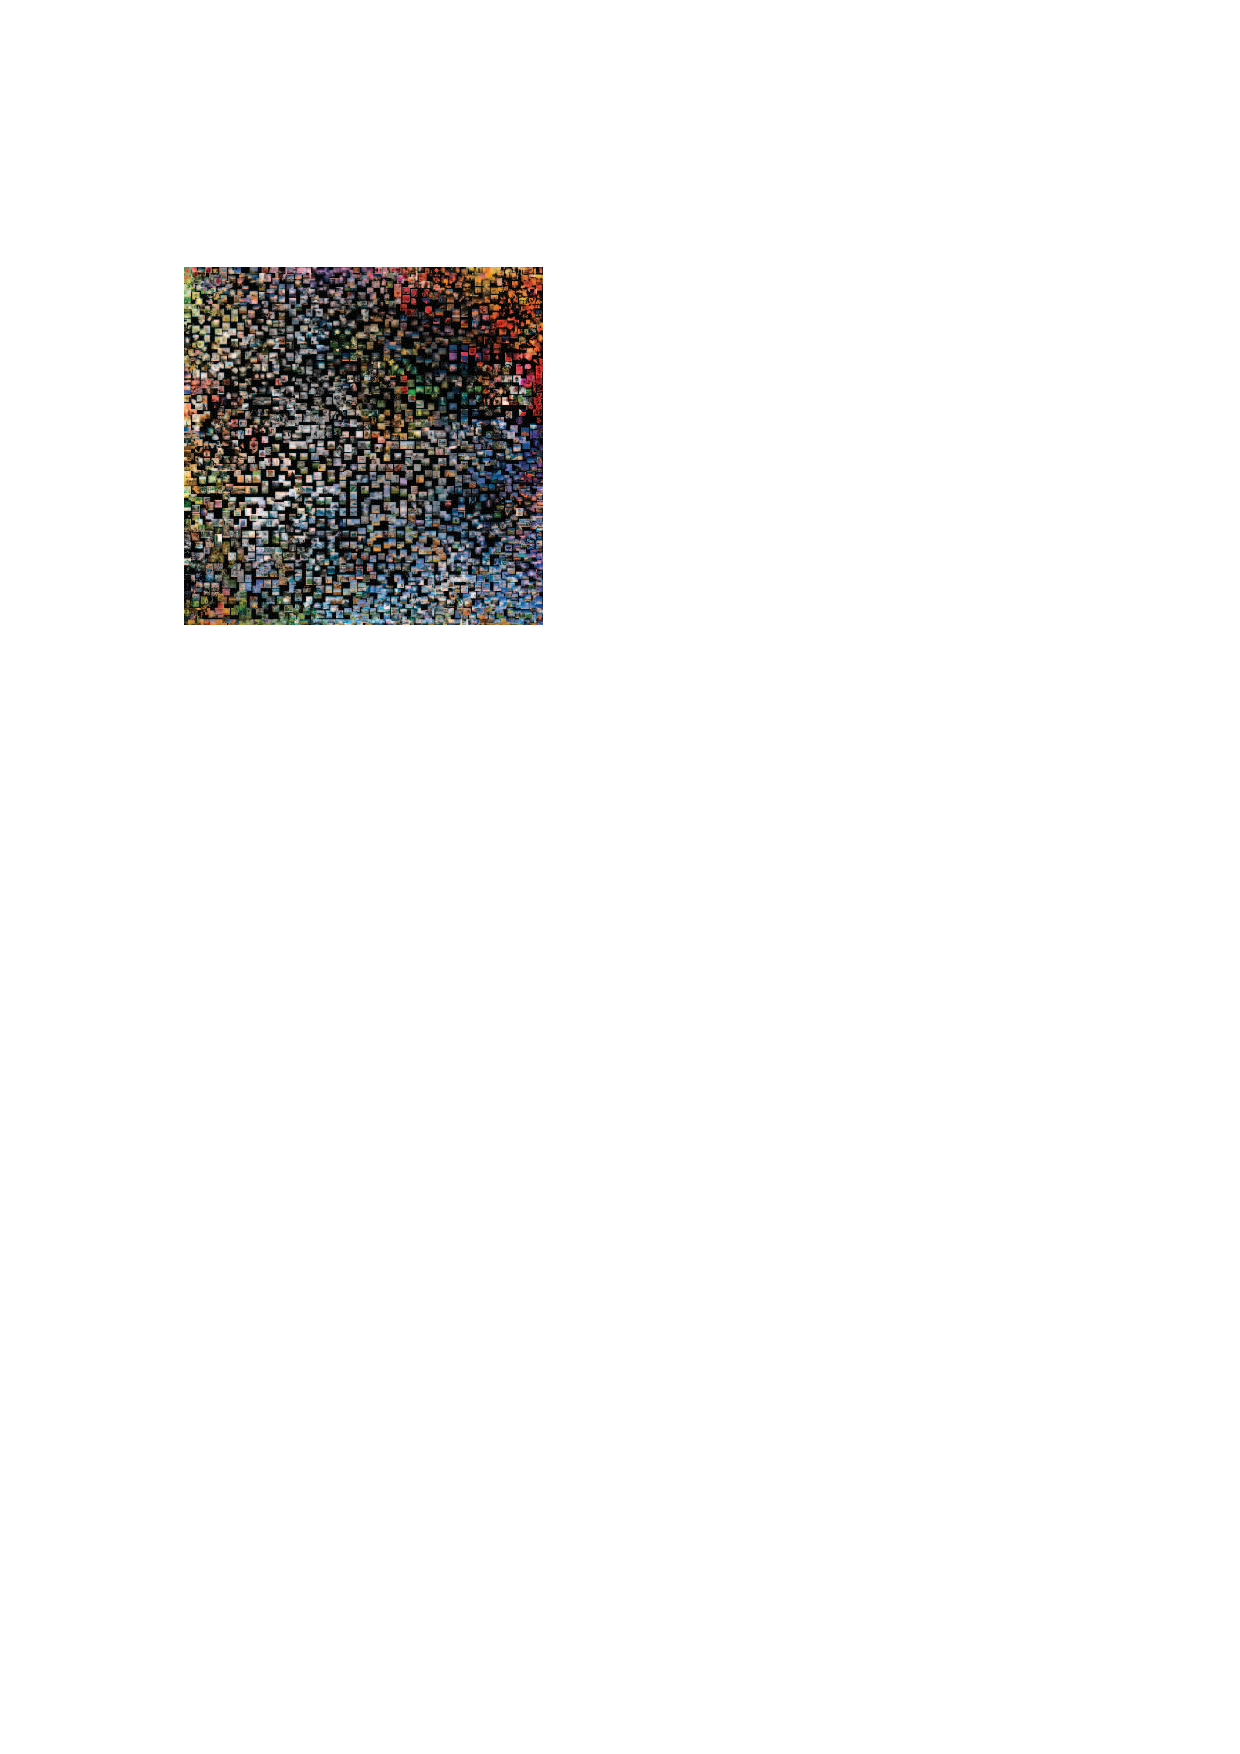
\includegraphics[scale=1]{imgs-RelatedWork/Strong1}
	\caption{The result obtained for organizing 2200+ photos using color autocorrelogram feature vector, using Strong's work \cite{Strong:2009p413}.}
	\label{fig:Strong1}
\end{figure}

% section strong (end)

\newpage
\subsection{An evaluation of color-spatial retrieval techniques for large image databases} % (fold)
\label{sub:Tan}
% não tem imagens

Tan et al. \cite{Tan:2001p850} present an evaluation of three color-spatial image retrieval techniques.

The signature-based technique creates a signature for each image, based on the most frequent colors, according to a threshold, of each subdivision, or bin, of that image. The comparison between images is made by comparing the main colors present on each bin. It is possible to assign more weight to specific bins according to the user's interest.

The partition-based approach is also based on bins, each having it's own color histogram. The similarity between images is given by the distance of the histograms of the corresponding bins.

The cluster-based method bases on the fact that humans focus on large patches (clusters) of the same color and, therefore, two images will appear similar if both have similar colored clusters on at roughly the same location. This method extracts the larger clusters and their color from each image. The similarity is calculated by the amount of overlap between clusters.

This techniques were tested with a collection of 12,000 images and, besides the color information, the brightness was also analyzed for increased performance. The authors conclude the signature method was generally better on both effectiveness and efficiency.

% section tan (end)

\subsection{Automatic organization for digital photographs with geographic coordinates} % (fold)
\label{sub:Naaman}

In this paper, by Naaman et al. \cite{Naaman:2004p1802}, is described a system that organizes digital photographs accordingly to location and date embedded on the metadata.

The objective was trying to mimmic the way people think about their collections. Photos are usually bursts separated by some time. Based on this and on the different places, events can be created to agglomerate photos from the same bursts. Location naming is done by calculating the most relevant places, like parks or cities, and then mixing the more precise locations with the more important neighbor cities to create a relevant and identifiable name. This was specially important since this work didn't involve showing any maps, but only the location names and events.

The authors showed good results and, nowadays, some common applications use similar features although including maps.
% section naaman (end)

\subsection{Similarity pyramids for browsing and organization of large image databases} % (fold)
\label{sub:Chen}

Chen et al. \cite{Chen:1998p2344} present a method for designing a hierarchical browsing environment called a similarity pyramid. The similarity pyramid groups similar images together while allowing users to view the database at varying levels of resolution. Each level is organized such that similar images are in close proximity on a two-dimensional grid (\fig{Chen1}). Images are first organized into a binary tree through agglomerative clustering based on color, edge and texture similarities. The binary tree is transformed into a quadtree, a tree in which each node has four children instead of only two.

\begin{figure}[ht]
	\centering
		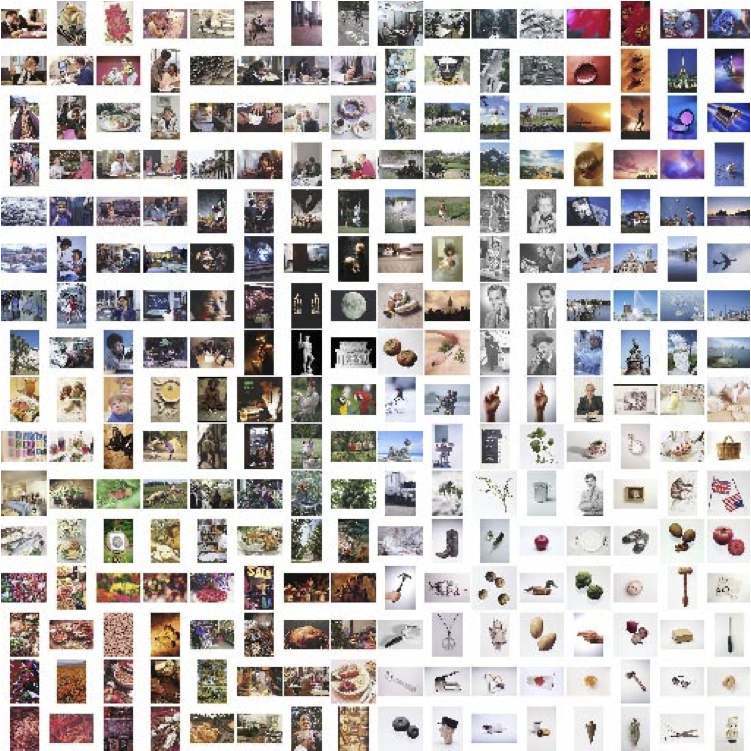
\includegraphics[scale=0.8]{imgs-RelatedWork/Chen-1998p2344.png}
	\caption{Images organized with \cite{Chen:1998p2344}. Images with similar color and texture are spatially adjacent.}
	\label{fig:Chen1}
\end{figure}

The similarity pyramid is best constructed using agglomerative (bottom-up) clustering methods, and a fast-sparse clustering method is presented which dramatically reduces both memory and computation over conventional methods. This method is based on the flexible agglomerative clustering algorithm, but using only a sparse proximity matrix and exploiting the author's approximate branch and bound search algorithm.

The authors found that the method for mapping the clustering to a pyramid can make a substantial difference in the quality of organization. Finally, a dispersion metric for objectively measuring pyramid organization was proposed, and found that it correlated well with the author's subjective evaluations of pyramid organization.

% section Chen (end)


\subsection{NN\super{k} networks for content-based image retrieval} % (fold)
\label{sub:Heesch}

Heesch \cite{Heesch:2004p2675} describes a different interaction technique for content based search in large image collections. Each image is a vertex in a graph and arcs are established between images if there exists at least one combination of features for which one image is retrieved as the nearest neighbor of the other. Each arc is weighted by the proportion of feature combinations for which the nearest neighbor relationship holds. By integrating the retrieval results over several feature combinations, the resulting network helps expose the semantic richness of images.

The interface reflects the vertexes and respective arcs, allowing to browse between the related images (\fig{heesch1}) in the network.

\begin{figure}[ht]
	\centering
		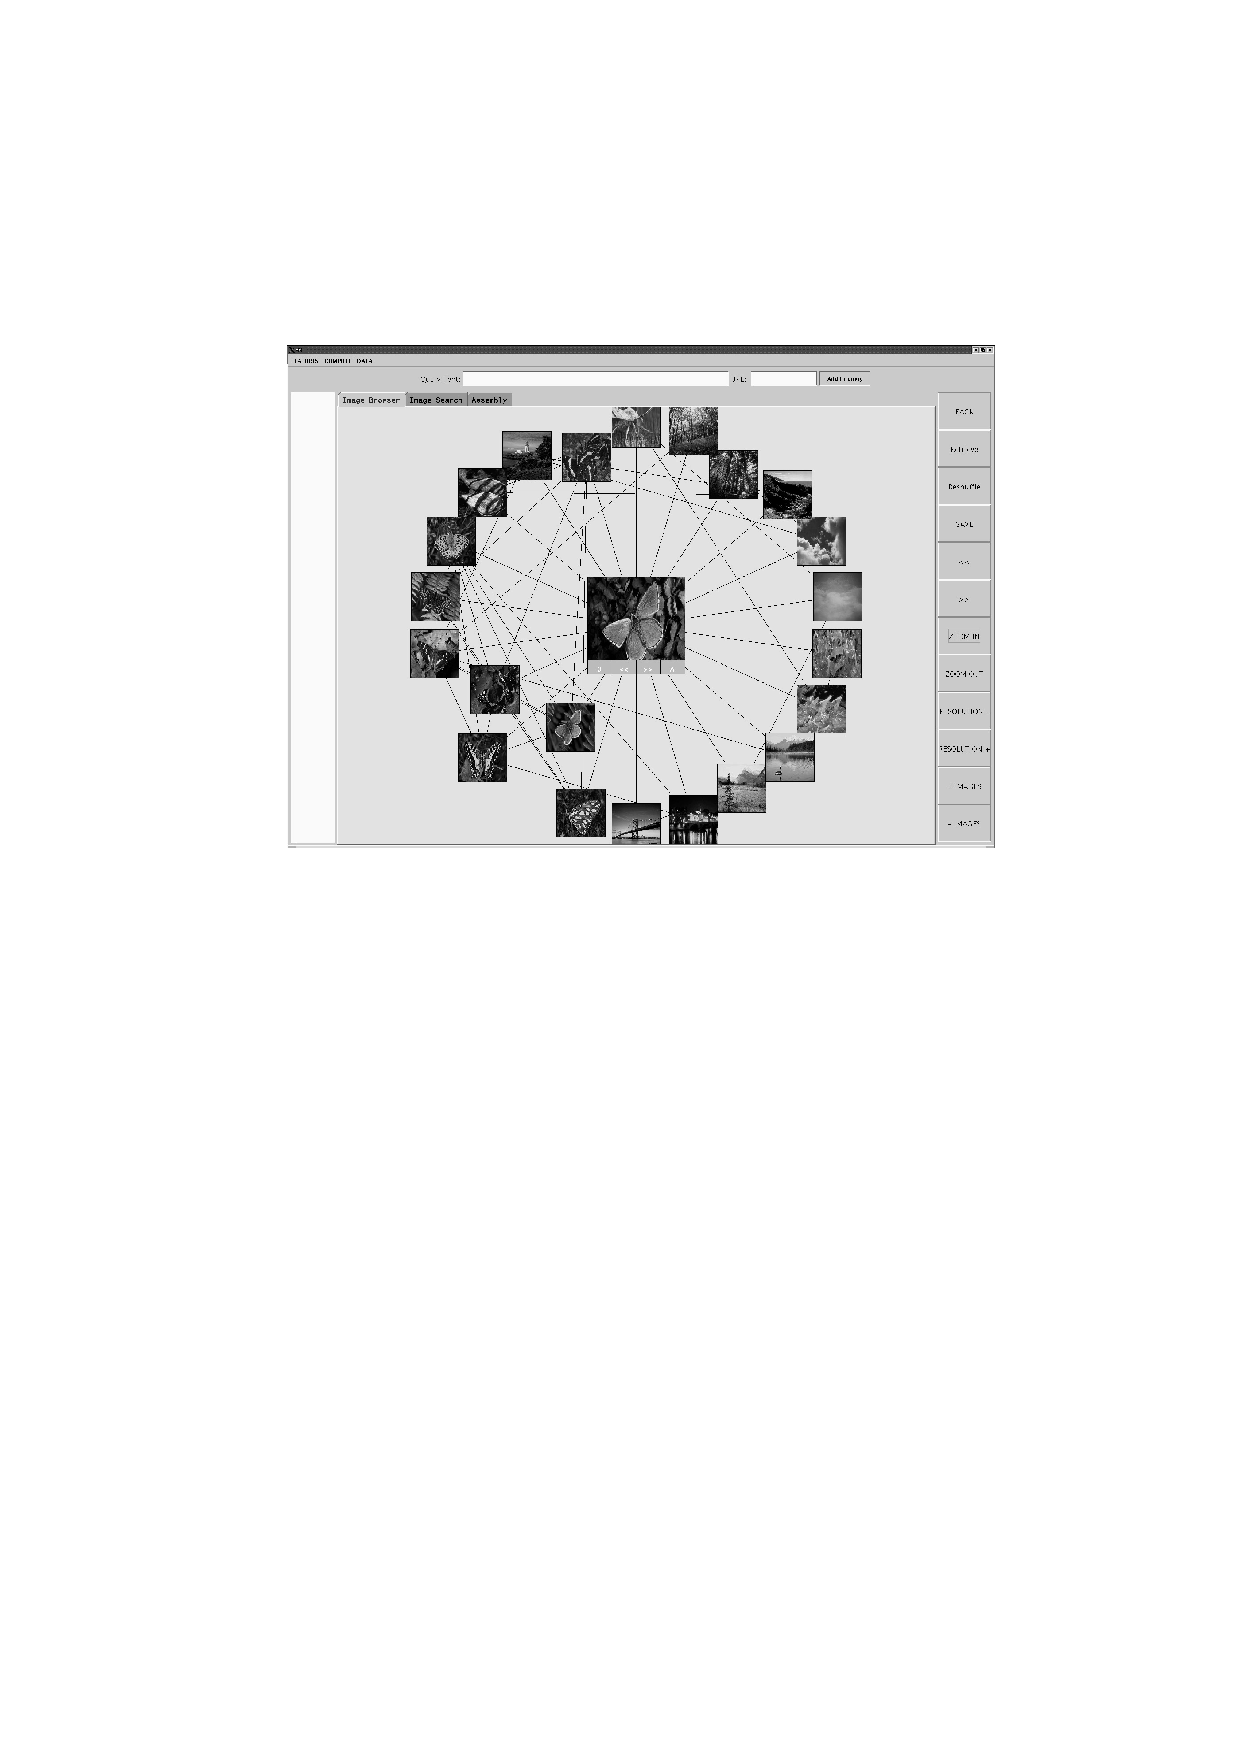
\includegraphics[scale=1]{imgs-RelatedWork/Heesch-2004p2675}
	\caption{Local network around the chosen butterfly image depicted in the middle.}
	\label{fig:heesch1}
\end{figure}

Seven low-level features are used for the classification of the images. HSV Global color Histograms maps the images by color, saturation and brightness; color Structure Descriptor maps the distribution of colors by dividing each image in 64 windows, the color space in 184 bins and associating color bins with image windows; Thumbnail feature compares identical images by saving the grey value of each pixel from a scaled down version of the image; Convolution filters discovers very selective features by reapplying 25 filters three times; Variance feature calculates standard deviations within a sliding window; Uniformity Feature is another statistical feature, calculating the grey level of an image split in 64 parts; Bag of words is the last feature and weights words associated to each image.

Tests showed great results when using a mix of search, relevance feedback and browsing, and even browsing by itself was considerably better than other, more restrictive, approaches.

The technique helps avoid the problem of image polysemy by showing all gathered meanings of the images to the user.
The feature network is pre-computed, allowing for quick realtime browsing. The authors claim it took 50 hours to process 32000 images, but made no reference to the possibility adding images to the collection, after the computation.

% section heesch:2004p2675 (end)

\subsection{Phorigami: A Photo browser based on meta-categorization and origami visualization} % (fold)
\label{sub:Hsu}

Hsu et al. \cite{Hsu:2009p2696} try to ease the browsing problem by analyzing the collections and identifying groups of related pictures. Each type of group is visualized in a specific way, inspired by the Origami art.

Groups of similar or related photos were manually classified based on camera movement and subject movement, creating different types of groups static view where both camera and subject are fixed and is presented as a panorama; multi-view where the subject is fixed, but the camera is moving and is shown as a presentation; if the subject is moving, the photos are categorized as motion capture and can be shown as an animated photo (fixed camera) or a presentation (moving camera); finally group photos, where different groups of people are photographed, are shown as a folding presentation.

This covers various cases where the photographer takes a few similar photos of the same subject because it's either a panorama, various angles or just to be sure the photo was well captured. 

The interface implements the different presentation types as different metaphors, easy for the user to understand, like a folded paper on a wide panorama that can be expanded (\fig{hsu1}). Although some of them appear to be a little hard to distinguish in its compressed form, it shouldn't be difficult to make it clearer. Other possible problem is the use of different touch interactions for each presentation type that might confuse users on what gesture should they use.

\begin{figure}[ht]
	\centering
		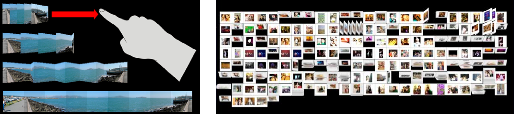
\includegraphics[width=\textwidth]{imgs-RelatedWork/hsu.png}
	\caption[Hsu's work of grouping together related images]{On the left, an example of an interaction on a group of photos that makes a panorama. On the right, a visualization on 537 photos with some groups.}
	\label{fig:hsu1}
\end{figure}


% section hsu:2009p2696 (end)

\subsection{A next generation browsing environment for large image repositories} % (fold)
\label{sub:Schaefer}

\begin{figure}[ht]
	\centering
		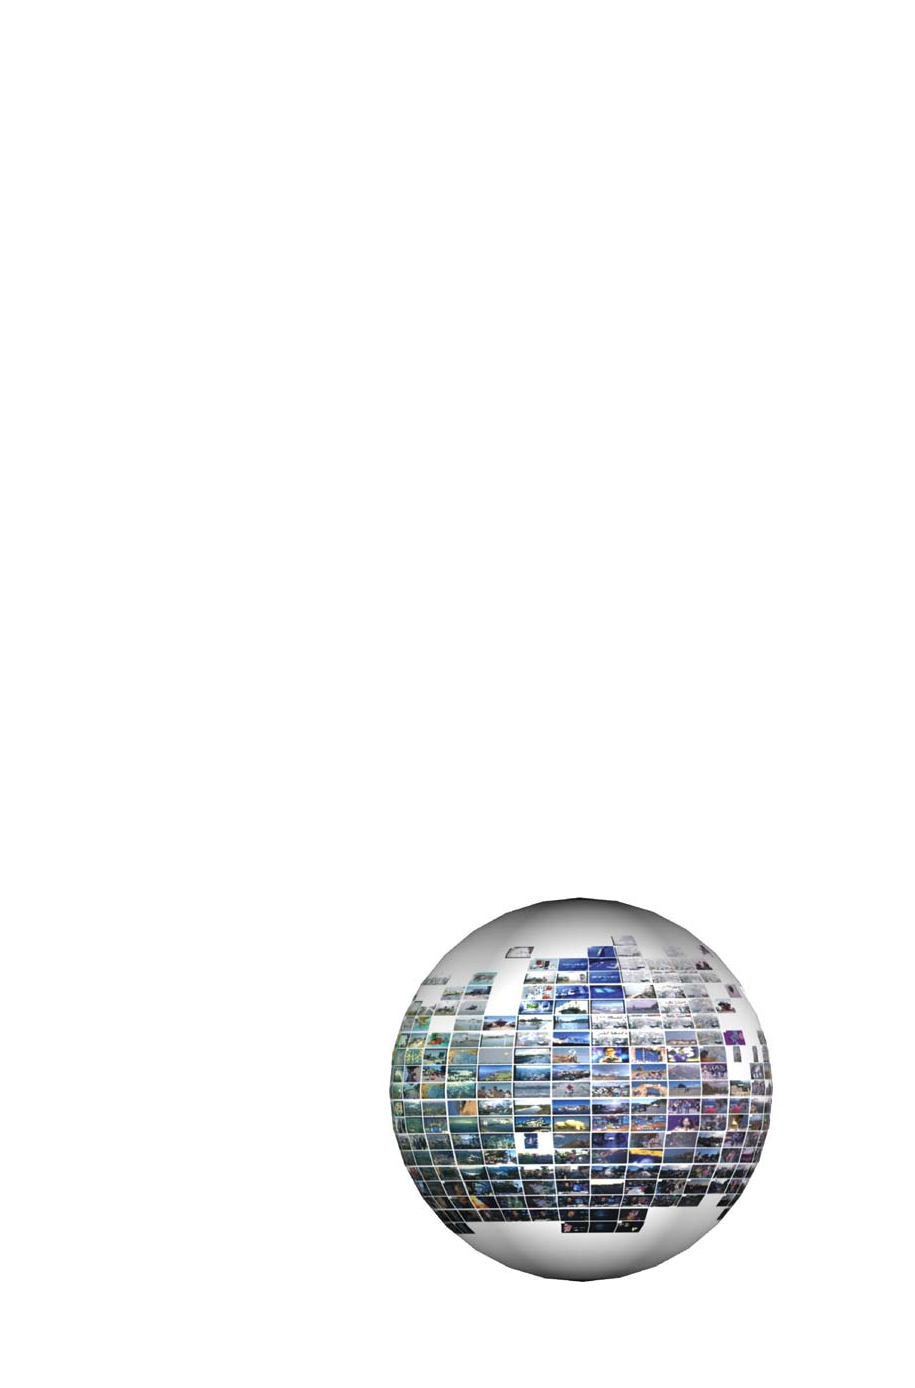
\includegraphics[scale=1]{imgs-RelatedWork/shaefer1.pdf}
	\caption{Hue sphere of a dataset, from Schaefer's work.}
	\label{fig:schaefer1}
\end{figure}

Schaefer \cite{Schaefer:2010p1871} tries to take similarity based organization of images from the 2D space to a 3D sphere, which allows interaction from the users. Rotating the sphere reveals images with different colors while tilting it reveals brighter or darker images.

Large image collections are handled through a hierarchical approach that brings up similar, previously hidden, images when zooming in on an area.

The description of the color is retrieved by calculating the image's median color for it's efficiency over other methods like histograms. This two features are directly mapped onto the sphere's coordinates and the entire structure is pre-calculated so browsing can be performed in real-time. Image overlapping is also avoided (\fig{schaefer1}).

The work was tested on a 4500 image collection with no evaluation as to its performance and a weak and subjective user testing.


% section schaefer:2010p1871 (end)

\subsection{Flexible access to photo libraries via time place, tags, and visual features} % (fold)
\label{sub:Girgensohn}
\begin{figure}[ht]
	\centering
		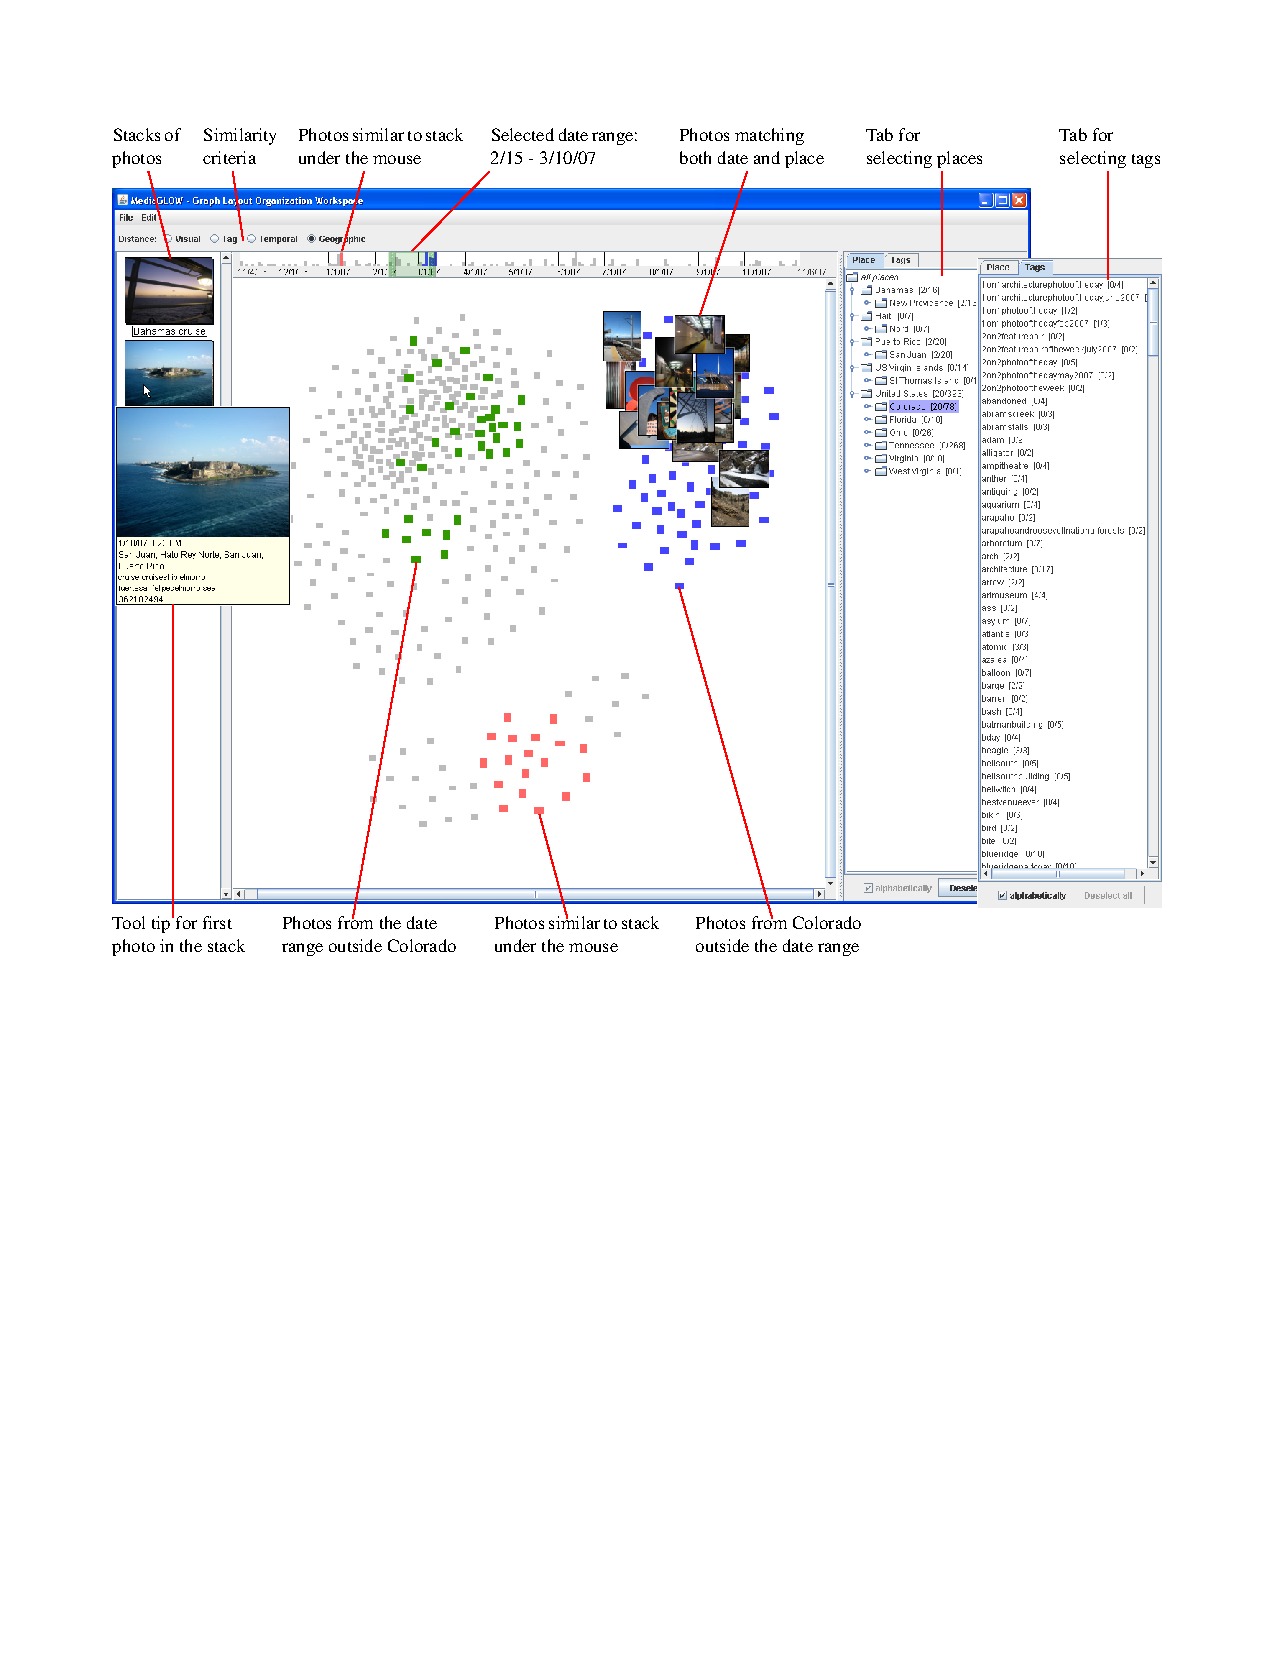
\includegraphics[width=\textwidth]{imgs-RelatedWork/Girgensohn1.pdf}
	\caption{Photos grouped by geographic similarity and filtered by date and place.}
	\label{fig:girgensohn}
\end{figure}

MediaGLOW by Girgensohn et al. \cite{Girgensohn:2010} is the application discussed in this paper. It's a \ac{CBIR} system with multiple ways to filter and sort the image collection.

The interface allows selecting a range of dates, places and tags at any time to filter the collection and the display will show the photos that match the filters, alongside indications of the existence of photos that match some of the filters. This display can then be arranged by four similarity criteria: temporal (by photo creation time), geographic (distances between places), tags (photos with similar tags are shown closer together) and visual (\fig{girgensohn}).

The time is selected using a timeline on the top of the screen while tags and places are shown on the right side sorted alphabetically, by frequency of, in case of places, as a tree. Multiple selections are allowed to show more photos.

The photo display is graph based, allowing for overlapped images. Various metaphors were developed to ease the navigation of the collection. Zooming is allowed and changes both thumbnail positions and size for better experience, allowing the photos to spread away from each other, but also increasing the size so the user can have a better look at them. The authors think that bigger thumbnails and a correct grouping of related photos is more important than spreading them to avoid the overlapping problem.

Color coding is used throughout the interface to help the user understand better what is being selected. For instance, on the timeline blue and grey are used to distinguish photos that match or not the selected location/tag. On the photo display, besides the photos that are actually shown are colored blocks: blue for photos that match location only, green for time only and grey for those that didn't match anything.

Detailed user testing was performed and the importance of the multiple ways to organize and search the collections was emphasized since many systems are designed to have a single form of access. Some users also pointed the importance of being able to have a non overlapping view of the photos for part of the task.

Each view was found to have different levels of usage, the geographic being the most used and temporal the least, since it's very similar to the timeline. Visual similarity was less used than expected, even on collections where it was relevant. 




\subsection{PhotoMesa: a zoomable image browser using quantum treemaps and bubblemaps}
\label{sub:PhotoMesa}

This work presents PhotoMesa by B. B. Bederson \cite{Bederson:2001:PZI:502348.502359}, an application that supports browsing sets of images in a zoomable environment. It also supports clustering by metadata, not requiring previous work from the user. Users can choose directories of images and they are all displayed in a space-filling manner \fig{photomesa}. Images are displayed in groups, from the directories they origin from and users can smoothly zoom in to a group and then to a single image. It generates multiple-resolution thumbnails for maintaing a good performance. Keyboard keys are also used to navigate the canvas. The groups display their name and have different background colors for a better distinction. It also supports drag and drop of images to other applications. Text search is possible as well as selecting a group on a list.

\begin{figure}[ht!]
	\centering
		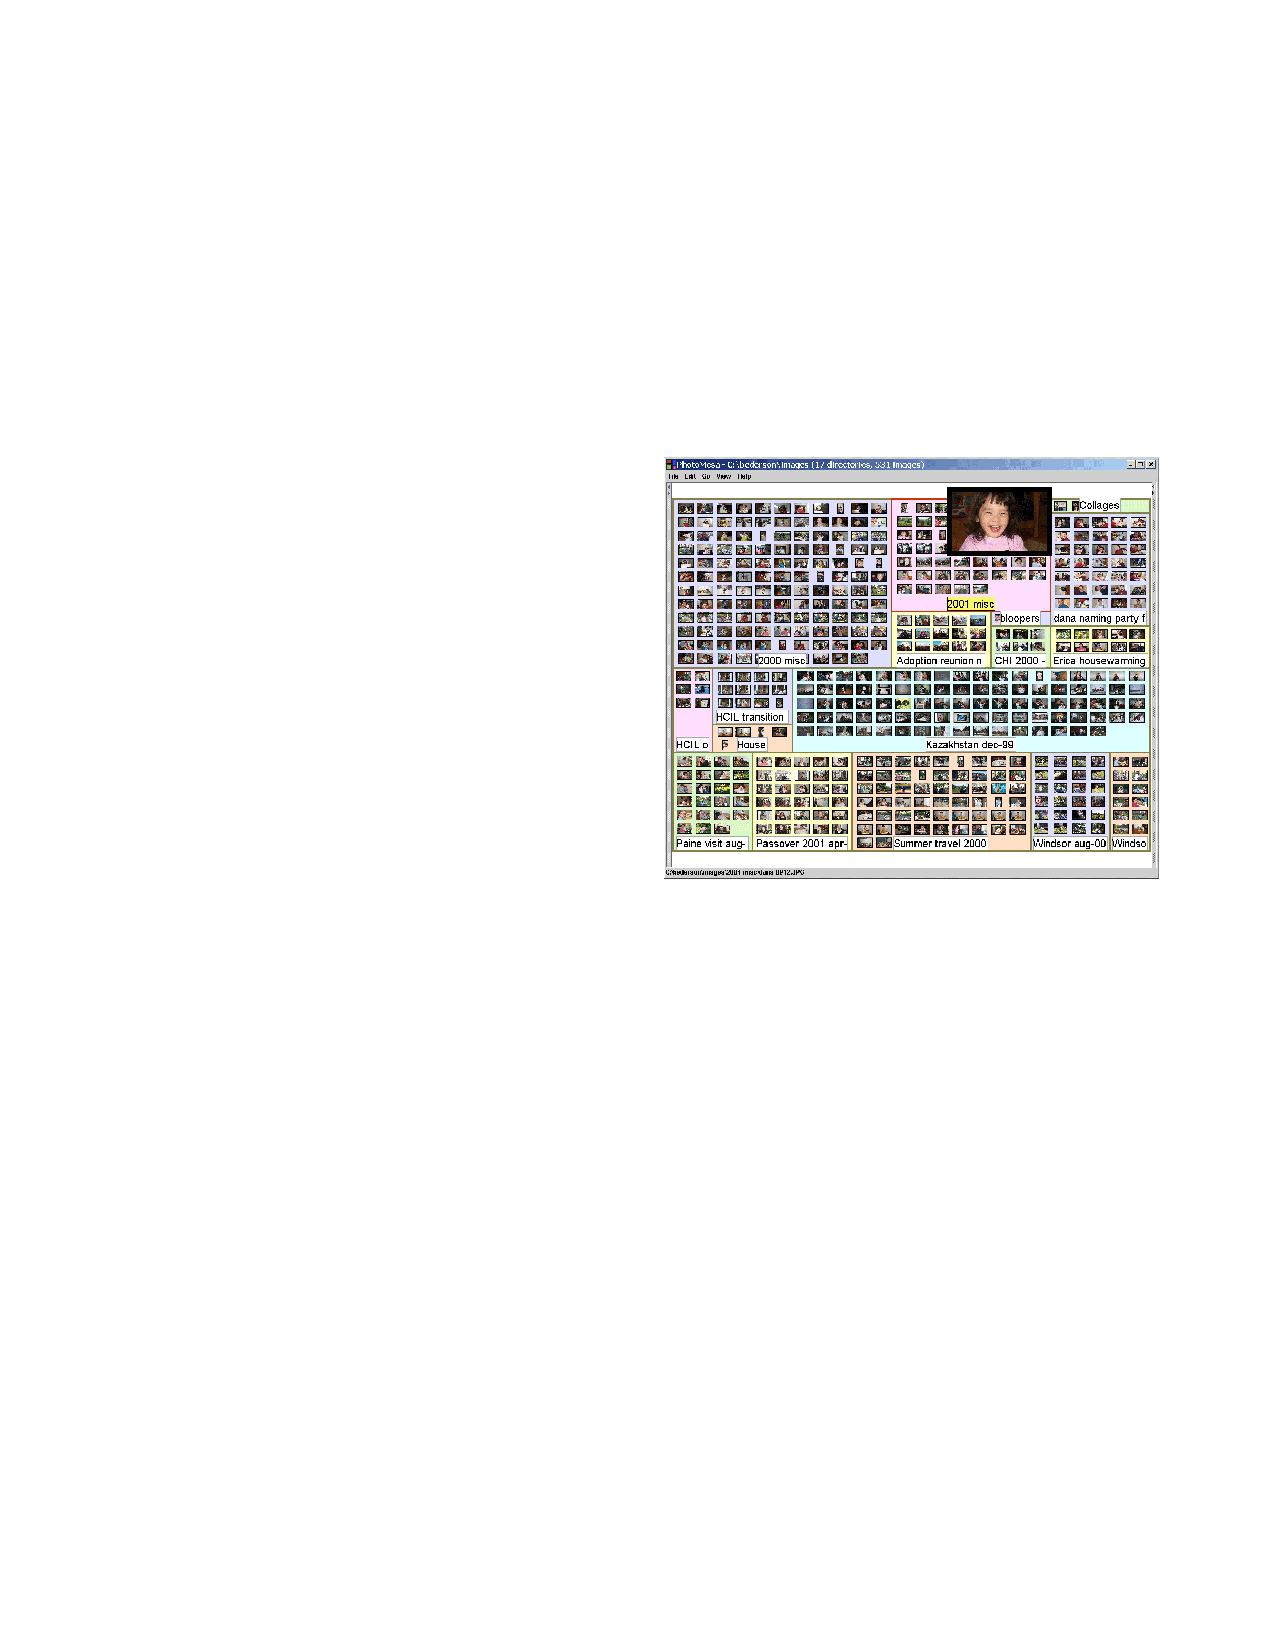
\includegraphics[width=0.90\textwidth]{imgs-RelatedWork/PhotoMesa.pdf}
	\caption{PhotoMesa with over 500 images in 17 groups.}
	\label{fig:photomesa}
\end{figure}

PhotoMesa implements two algorithms for space filling, one is Quantum Treemaps by the author, a variation of the Ordered Treemap  that is aware of the constraints imposed by the use of images, like grid alignment and common size, and Bubble Maps which is designed to have the least wasted space possible.

This work brings very interesting ideas to the table, but it has a somewhat limited reach, with only referring to ``over 500 images'' on the application and by only taking simple metadata, like the path and modification date of images.




% section girgensohn:2010 (end)

\section{Discussion} % (fold)
\label{sub:discussion}


Currently there are a lot of approaches to image organization and each has its own differences as demonstrated on Table \ref{tab:brows-meth}. Our survey went by multiple works and revealed various methods for extracting the features from each image, multiple visualization methods from grids to flying images.


\begin{table}[ht]
 \begin{tabular}{| m{2.7cm} |>{\centering}m{2.3cm}|c|c|c|>{\centering}m{2.1cm}|>{\centering}m{2.3cm}|r|}
  \hline
\multirow{2}{*}{\textbf{Work}} & \multicolumn{4}{c|}{\textbf{Organization}} & \multirow{2}{*}{\textbf{Visualization}} & \multirow{2}{*}{\textbf{Focus}} & \multirow{2}{*}{\textbf{Size}} \\
\cline{2-5}
	& \textbf{features} & \textbf{date} & \textbf{gps} & \textbf{tags} & & & \\

\hline 1.	Qiu \cite{Qiu:2007p1207}	& simple color measures 			& --- & --- & --- & Grid 			   & Simplicity and Efficiency 			& 60,000	\\
\hline 2.	Rodden \cite{Rodden:2001p731}	& --- 								& --- & --- & \cm & Grid 			   & Similarity usefulness	 			& 	 100	\\
\hline 3.	Porta \cite{Porta:2006p416}	& --- 								& --- & --- & --- & Spot (and others)  & Unconventional visualizations		& 	 400	\\
\hline 4.	Cooper \cite{Cooper:2006p543}	& --- 								& --- & --- & --- & Static and animated& Usefulness of animations 			& 	 ---	\\
\hline 5.	Strong \cite{Strong:2009p413}	& color histograms and gradients 	& --- & --- & --- & \ac{SOM} 		   & Evaluation of different features	&  2,200 	\\
\hline 6.	Tan	\cite{Tan:2001p850}		& color histograms of subdivisions & --- & --- & --- & --- 			   & Evaluation of different features 	& 12,000 	\\
\hline 7.	Naaman	\cite{Naaman:2004p1802}	& --- 								& \cm & \cm & --- & --- 			   & Organization based on events 		& 	   N/A	\\
\hline 8.	Chen	\cite{Chen:1998p2344}	& colors, edges and textures 		& --- & --- & --- & --- 			   & Efficient fast-sparce clustering 	& 10,000 	\\
\hline 9.	Heesch	\cite{Heesch:2004p2675} & six different features 			& --- & --- & \cm & Radial 			   & Complex similarity network 		& 32,000 	\\
\hline 10.	Phorigami, Hsu	\cite{Hsu:2009p2696}	& --- 								& --- & --- & --- & Grid with groups   & Interaction on grupped photos 		&  1,333 	\\
\hline 11.	Schaefer \cite{Schaefer:2010p1871} & color histograms of subdivisions & --- & --- & --- & 3D Sphere		   & 3D mapping and interaction 		&  4,500 	\\
\hline 12.	MediaGLOW, Girgensohn \cite{Girgensohn:2010}	& --- 								& \cm & \cm & \cm & Overlapped graph   & Having the best way to find photos &    450	\\
\hline 13. PhotoMesa, Bederson \cite{Bederson:2001:PZI:502348.502359} & --- & \cm & --- & \cm & Q. Treemap / Bubblemap & Zoomable browser & 500	\\
\hline
 \end{tabular}
\caption{Different browsing methods}
\label{tab:brows-meth}
\end{table}

One of the main problems is obtaining useful information from low level feature extraction of the image contents. Some try to get the most out of each image, with a variety of complex and time consuming procedures, e.g., a variety of methods based on color histograms \cite{Strong:2009p413,Tan:2001p850,Chen:1998p2344,Schaefer:2010p1871} or even more detailed ones with textures and convolution filters \cite{Heesch:2004p2675}. Others try to focus on avoiding the complex computations by only getting simple, but somewhat useful information \cite{Qiu:2007p1207}. To contrast with these methods, Girgensohn's work \cite{Girgensohn:2010} has found that users prefer other ways to filter the collection, like tags, dates and locations. Low level features are still used, but they have to be kept to understandable and useful options.

Date and location are simple similarity measures and can be used to group the collections by events and locations like Naaman did on this work \cite{Naaman:2004p1802}. Current mainstream software like Apple's iPhoto\footnote{http://www.apple.com/iphoto} or Google's Picasa\footnote{http://picasa.google.com} are already doing it in a semi-automatic way.

Textual metadata like tags and descriptions are also widely used both on our survey \cite{Rodden:2001p731,Girgensohn:2010,Heesch:2004p2675,Bederson:2001:PZI:502348.502359} and on all mainstream software. The problem with tags and descriptions is that people usually don't assign them to their photos, but that's not a problem we're interested here.

The visualization is the field with most variations and experimentations, like Porta's work \cite{Porta:2006p416} where multiple options were tested, but only a couple of the most simple were considered useful. The 3D Sphere \cite{Schaefer:2010p1871} is also visually interesting, but doesn't provide a better interface to the collection since it's based on a grid view, but hiding many images on the far side of the sphere. The Phorigami work \cite{Hsu:2009p2696} introduces some interesting metaphors for reducing the space occupied by some groups of photos, but some make the visualization harder and could, therefore, be improved.

Girgensohn and Bederson's works are among the most interesting and relevant to our vision. MediaGLOW's \cite{Girgensohn:2010} visualization approach allows images to be organized by various features and to be filtered down, displaying matched photos alongside placeholders for photos that are only match partially. The timeline on the top is also very useful. It has some problems like image overlap and capacity for showing large collections, but the ideas are still interesting. PhotoMesa \cite{Bederson:2001:PZI:502348.502359} has a visualization style close to what we want from our work, but its reach is short, i.e., has a small set of features and dispositions, doesn't handle many images and the \ac{UI} seems a little cluttered with all the strong colors and borders.

The seemingly more useful exploration tools are the ones that handle less images, which seems like a contradiction. The more images a system can hold and efficiently display, the more useful it gets. From our user survey (appendix \ref{appendix:usersurvey}), we learnt two thirds of people have less than 10 000 photos (\ref{ssub:library_size}) and we will do our best to reach that level.

% section discussion (end)
% chapter related-work (end)